% ESE650 Learning in Robotics - Project 4

\documentclass{article}
\usepackage{graphicx}
\usepackage{color}
\usepackage{listings}
\usepackage{fullpage}
\usepackage{amsmath}
\usepackage{placeins}

\definecolor{lightgray}{gray}{0.5}
\setlength{\parindent}{0pt}
\setcounter{secnumdepth}{0} %turn off section numbering
\begin{document}

\title{ESE650 Project 4: Simultaneous Localization and Mapping}
\author{Joe Trovato}
\date{\today}
\maketitle
\setlength{\parindent}{10ex}

\section{Introduction}
Simultaneous Localization and Mapping (SLAM) is a core problem in robotics. The ability to sense the surrounding environment and determine where the robot is within that environment is essential to a variety of tasks. In this project, I implemented a basic SLAM algorithm using a particle filter to track location and an probabilistic occupancy grid to keep track of the map. Once SLAM was working (to an acceptable level of accuracy), I used the RGB data taken from the camera to map color to the floor displayed in my occupancy grid. 

\section{Algorithm}
\subsection{Data Preprocessing}
The dataset given contained a variety of information, most of which  I did not incorporate into the project. My implementation uses the lidar readings, the head and neck joint angles, the IMU readings and their respective time stamps. For the final part of the project I used the RGB data contained in the kinect data file to map color to the floor. 
 
\subsection{Mapping}

\subsubsection{Occupancy Grid}
After experimenting with naive algorithm for a binary occupancy grid, I implemented a logistic occupancy grid which tracked a probability of being occupied for each grid square. As discussed in class, instead of storing raw probability values in the grid data structure, I stored the domain value of a sigmoid function. This make it easier to increment or decrement the probability of a space being occupied, because a constant value can either be added or subtracted. The form of the sigmoid function (See figure 1) ensures that values close to zero are less confident than those farther away from zero.
\FloatBarrier

\begin{figure}[!h]
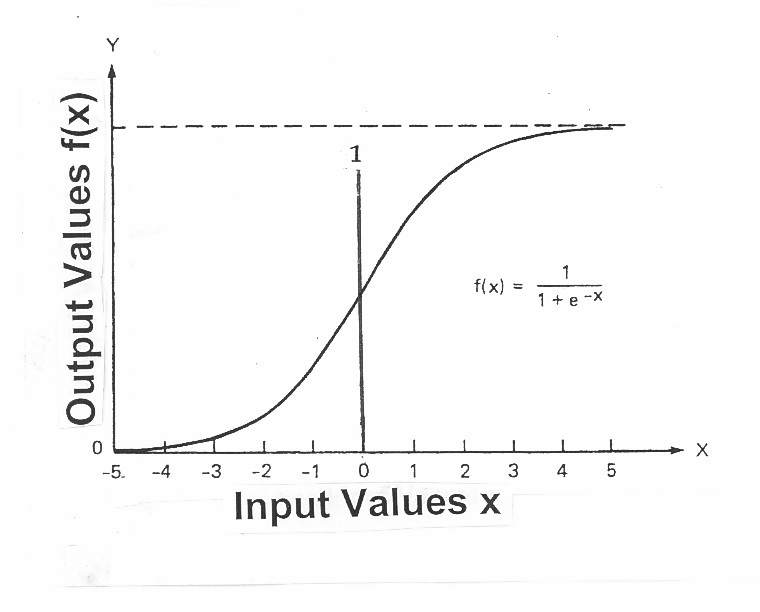
\includegraphics[width = 0.6\textwidth]{sigmoid.jpg}
\centering
\caption{sigmoid function used to generate probabilities from occupany grid values}
\end{figure}

\FloatBarrier

\subsubsection{Lidar Transformations}
\par
The mapping algorithm uses the lidar hits to determine where object in the environment are. The lidar is mounted on the head of the robot but our occupancy grid only tracks $x$, $y$, and $\theta$. This requires making a transformation from the lidar's coordinate system to the global cordiante system. This transformation was acheived by cascading homogeneous transformation matrices between different reference frames. The lidar point are transfromed from the head to the neck, then from the neck to the body, then from the body to the world, yeilding three homogeneous transforms. Using zero as the z-component of all lidar hits and augmenting the coordinate vector with a one gives lidar hits in homogeneous coordinates, the form needed for this transformation.

$$ ^{World}H_{Lidar} = ^{World}H_{Body} \times ^{Body}H_{Neck} \times ^{Neck}H_{Lidar}  =  ^{World}[R,t]_{Body} \times ^{Body}[R,t]_{Neck} \times ^{Neck}[R,t]_{Lidar} $$

Where $R$ is a rotation matrix and $t$ is a translation vector. 
\\
\\
\par
Once the lidar hits are expressed in real world coordinates the occupancy probability of the grid squares that correspond to the lidar hit are incremented and the grid spaces in between the robot and that point are decremented. I found these points use the raytracer mex file provided. 
\par
In addition to this basic implementation, a few tricks were employed to get the best performance from the map. The first was enforcing a limit on the probabilities. Without a limit, if a point is seen as 'free' for many iterations, it will be difficult to convince the algorithm that a object is their when a new object is introduced. In this way, the map can more easily update based on a dynamic environment. Another trick was changing the the the value of the increments. My occupied increment is ten times larger than my free decrement because it is much more likely to see a free space than a lidar hit due to the ray tracing algorithm. 
\par
As Figure 2 shows, the map is color coded in grayscale. This was chosen to save memory when dealing with the map. Gray represent a grid value of 0 and 50\% chance of being occupied, or more meaningfully that we haven't seen any data for it. lighter gray and white represents free space and black represents occupied space or obstacles in the environment. The robot is represented by a green triangle where the point is in the direction of $\theta$.

%insert a figure here of a map
\FloatBarrier

\begin{figure}[!h]
\includegraphics[width = 0.6\textwidth]{ESE650_Proj4/map2.png}
\centering
\caption{An example of map generated by my SLAM algorithm}
\end{figure}

\FloatBarrier

\subsection{Localization}
\par
The odometery data provided in the dataset is an extremely poor representation of the actual path taken by the robot. When plotting the map using the actual odometry data, the map often drifts and rotates according to noise in the odometry. To fix this a particle filter was used.
\subsubsection{Particle Filter}
\par
A particle filter is used to track the location of an agent by selecting the most probable state from a group of possible particles each with a different state. The probabilities or weights are determined by how much the current position and current lidar hits are consistent with the map.
\par
My implementation was more basic than a traditional particle filter. A particle filter normally introduces noise into the state variables ($x$,$y$,$\theta$) and tracks them from iteration to iterations, resampling when needed. My system used a school of fish method of introducing noise. So for each iteration a new particle was placed in all of the surrounding grid spaces up to a certain radius. I found that two was a good radius. Finally noise in theta was generated by sampling angles drawn from a gaussian distribution centered at the previous theta value. The particle which has the highest lidar map correlation is then chosen as the true location of the robot. By throwing away the all particles other than the believed state of the robot allows for faster run times and less complicated updates.

The majority of the issues I ran into were concerned with the  particle filter. Tuning the noise introduced into the particle was key in developing a good map. I found that the more particles the better map was. This makes sense because with more particles, there is a higher change of a particle being at or very close to the true location.
\par
Another issue was the propensity of the robot to slip forward. This mean that the particle directly in front of the robot should be more likely than the other particles. To encode this, I introduced a prior into the scores for those particle directly in front of the robot current believed state.

\section{Results}
I have attached a video of the algorithm running on a training set as well as another video for the test set. 


\section{Demo Instructions}
\begin{enumerate}
	\item Specify test files for lidar and joints by editing files names at top of SLAM.m
	\item change dataset variable at top of SLAM.m to correct number
	\item run SLAM.m, map should display

\end{enumerate}


\end{document}